\chapter{Sistemas relacionados}

Em uma geração dirigida pela tecnologia e engajamento em causas sociais é possível perceber que várias aplicações têm sido criadas em todo o mundo no cenário da violência contra a mulher.

No Brasil, alguns aplicativos e sites surgiram como consequência de políticas públicas. Como o site Minha Voz \footnote{Minha Voz \url{http://minhavoz.com}} e os aplicativos Clique180, SalveMaria, SOSMulher e Lei Maria da Penha.

Outros aplicativos e sites foram criados pela própria população, como: Vazow, Juntas, Chega de Fiufiu, 
SaiPraLá, PLP 2.0, Assédio Zero e Mete a Colher.

\section*{Minha Voz}

Site criado no \textit{Hackathon} de Gênero e Cidadania, no qual
um dos temas era "Violência Contra a Mulher". 

De acordo com a documentação do site (disponível no GitHub\footnote{Repositório Minha Voz \url{https://github.com/saletefarias/Minha-Voz}}), o objetivo é ter um fórum para apoio às mulheres, no qual elas podem
realizar desabafos e obter um panorama da violência contra a mulher através de um questionário
disponível no site relacionando os dados por:

\begin{itemize}
	\item Categorias;
	\item Locais;
	\item Grau de Proximidade com o agressor;
	\item Tempo de duração da violência;
	\item Data.
\end{itemize}

O site também disponibiliza um questionário para que a mulher possa identificar a categoria (tipo) da violência sofrida, respondendo à perguntas pré-definidas com "Sim" ou "Não". Esse questionário é construído baseado em uma árvore de decisão.

\vfill

\section*{Clique180}

Trata-se de um aplicativo para Android criado pelo Onu Mulheres que, de acordo com
a página de download\footnote{Clique180 \url{https://play.google.com/store/apps/details?id=br.com.negociosreais.sosmulher&hl=pt_BR}}, oferece:

\begin{itemize}
	\item Leis e conceitos;
	\item Localização Rotas até os serviços da rede de atendimento às mulheres;
	\item Botão para ligação para o 180;
	\item Dicas de ações a serem tomadas e tipos de serviços a procurar; 
	\item Mapeamento de locais de risco.
\end{itemize}

\section*{SalveMaria}

Criado pelo governo do estado do Piauí, o SalveMaria\footnote{SalveMaria \url{https://play.google.com/store/apps/details?id=br.gov.pi.ati.salvemaria&hl=pt_BR}} é um aplicativo para envio de denúncias
de forma sigilosa, informando o tipo de assédio sofrido.
Além disso, conta com um Botão do Pânico que envia um pedido de socorro automaticamente para a polícia.

\section*{SOSMulher}

Aplicativo, criado pelo governo do estado do Pará, para mulheres que estão sob medida protetiva. 
De acordo com notícia publicada\footnote{SOSMulher \url{http://g1.globo.com/pa/para/noticia/2016/03/aplicativo-sos-mulher-aciona-ajuda-em-caso-de-violencia-no-pa.html}}, o aplicativo é instalado no \textit{smartphone}, e quando a mulher está em situação de risco, por meio de três toques no aparelho, são enviadas notificações para a Central da Guarda Municipal.

\section*{Lei Maria da Penha}

Criado pelo Programa internacional de promoção da igualdade de gênero, raça e etnia, trata-se de um
aplicativo que contém toda a Lei Maria da Penha.

\section*{Vazow}

Aplicativo para Android para vítimas de vingança pornô, do inglês "revenge porn", que é a 
divulgação de vídeos e/ou fotos íntimas após término.
De acordo com a página de download\footnote{Vazow \url{https://play.google.com/store/apps/details?id=xdk.intel.blank.ad.template23&hl=pt_BR}}, as funcionalidades oferecidas são:

\begin{itemize}
	\item Procedimentos e orientações para exclusão de conteúdo íntimo divulgado;
	\item Dicas de como evitar se tornar uma vítima;
	\item Legislação relacionada;
	\item Suporte para contato.
\end{itemize}

\section*{Juntas}

O site Juntas é um blog que contém \textit{posts} informativos, conceituais e notícias 
relacionadas ao cenário feminino no Brasil.

\section*{Chega de Fiufiu}

Um site no qual a mulher pode realizar uma denúncia de uma violência sofrida ou presenciada. 
Essa denúncia é realizada informando o endereço, o tipo de violência sofrida, a data, período do dia e o que foi feito. De acordo com o site\footnote{Chega de Fiufiu \url{http://chegadefiufiu.com.br/}}, o objetivo é "mapear os lugares mais incômodos e até perigosos para mulheres no Brasil".

\section*{SaiPraLá}

Aplicativo para realização de uma denúncia de violência informando o endereço em que o assédio ocorreu, o período do dia, o tipo de assédio e o que foi feito. De acordo com a a página de download\footnote{SaiPraLá \url{https://play.google.com/store/apps/details?id=br.com.saiprala&hl=pt_BR}}, o objetivo é "mapear o assédio e atuar na prevenção dele".

\section*{PLP 2.0}

Aplicativo que possui um detector de emergência para acionar diretamente as redes de atendimento 
e também realiza a gravação de áudios e vídeos\footnote{PLP 2.0 \url{https://play.google.com/store/apps/details?id=br.com.beelieve.plp&hl=pt_BR}}.

\section*{Assédio Zero}

Aplicativo para as mulheres denunciarem dois tipos de agressão: física ou verbal, marcando a localização 
onde a violência ocorreu. Assim como os outros aplicativos de denúncia, o Assédio Zero\footnote{Assédio Zero \url{https://play.google.com/store/apps/details?id=br.com.assediozeroapp&hl=pt}} tem como objetivo mapear a violência contra a mulher.

\section{Considerações finais}

Considerando as informações de cada sistema, foi possível perceber que as aplicações têm funcionalidades
em comum e assim estabelecer cinco categorias de funcionalidades: Levantamento de Dados e estatísticas, Mapeamento de riscos, Informativos , Pedido de Socorro e Denúncia. 

Na categoria de Levantamento de Dados e estatísticas foram mapeadas as aplicações que possuem
o intuito de obter dados estatísticos sobre a violência de acordo com as respostas/denúncias das mulheres.

A categoria de Mapeamento de riscos também trata das aplicações que obtém os dados de violência através
das respostas/denúncias das mulheres, porém com o objetivo de mostrá-las os locais de risco.

As aplicações com funcionalidades relacionadas à disponibilização de leis, informações e conceitos foram
categorizadas em Informativos.

As aplicações com finalidade de pedido de socorro automático foram categorizadas em Pedido de Socorro. E por fim, na categoria de Denúncia, estão as aplicações que tem funcionalidade para realização de denúncias de violência

Na Figura \ref{fig:sistemas_categorizados} é apresentado o mapeamento das aplicações com as categorias criadas.

\begin{figure}[h!]
\centering
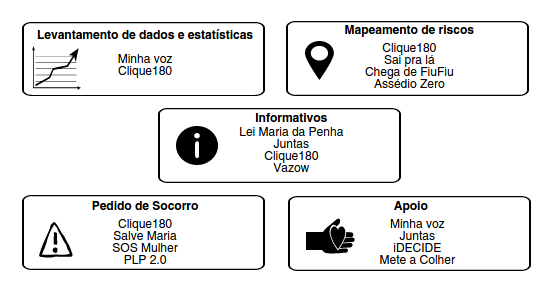
\includegraphics[scale=0.75]{figuras/sistemas_relacionados.png}
\caption{Aplicações de apoio à mulher vítima de violência}
\label{fig:sistemas_categorizados}
\end{figure}

Em suma, as aplicações no geral auxiliam nas denúncias, gerando dados como locais de riscos e estatísticas e
apresentam informações genéricas sobre como agir em situações de violência. Dessa forma, percebe-se uma lacuna em um apoio mais específico de acordo com a situação de violência vivida pela mulher.

% , como sugestões de ações a serem tomadas e planejamento de segurança, como por exemplo, a proposta do I-DECIDE.

% Em 2011, o Laboratório Hacker da Câmara dos Deputados promoveu um \textit{Hackathon} de Gênero e Cidadania, no qual
% um dos temas era "Violência Contra a Mulher". O site Minha Voz foi o vencedor e de suas funcionalidades é um questionário que ajuda a mulher a identificar o tipo de violência sofrida. 

% Na Figura \ref{fig:sistemas_categorizados} são apresentadas algumas aplicações criadas no Brasil para apoio à mulher vítima de violência categorizadas em cinco tipos: Levantamento de Dados e estatísticas, Mapeamento de riscos, Informativos, Pedido de Socorro e Apoio.

